\chapter{Comparative data}
\label{ch:Comparative data}

\section{Gros et al paper}
\indent This project was largely based on the paper published by S. Gros \textit{et al.} \cite{SG09} outlining performance tests for planar germanium detectors. The paper provided many benchmarks for detector evaluation and explanation of some of the common problems seen in DSSDs. Tests for Ge DSSDs were grouped according to the number of pixels involved in the gamma event. Some tests were performed only with one hit events while others required two pixels. A number of different high-purity Ge detectors were examined in the Gros paper, including one coaxial LEPs, two planar strip detectors with lithium and boron contacts, and two planar strip detectors with amorphous Ge contacts. (Explain more about detectors used?) The Mark 3 detector used in the Gros paper is the Ortec detector used in this master's project.

\subsection{Single Pixel Tests}
\indent The first, and arguably most important, test was resolution of each strip as measured by a single channel MCA. Measuring the resolution of each detector was done one strip at a time while the other strips were not connected to any electronics. This was done to minimize any equipment-based cross talk or grounding problems.\cite{SG09} As demonstrated in the Gros paper, it is common to see that large, segmented detectors actually have worse resolution than LEPS detectors. A plot of the resolution across the face of the detector should ideally show all strips having nearly the same resolution.  Poor resolution on the edge strips can be a sign of an inadequate guard ring. \cite{SG09} Below are the lower-energy parts of a $^{152}$Eu spectrum collected by the LEPS detector and the amorphous contact planar detector as seen in the Gros paper. As predicted, the LEPS detector clearly has better resolution than the planar strip detector. 

\begin{figure}[h!]
  \centering
%  \setlength\fboxsep{0pt}
%  \setheight\fboxsep{0pt}
  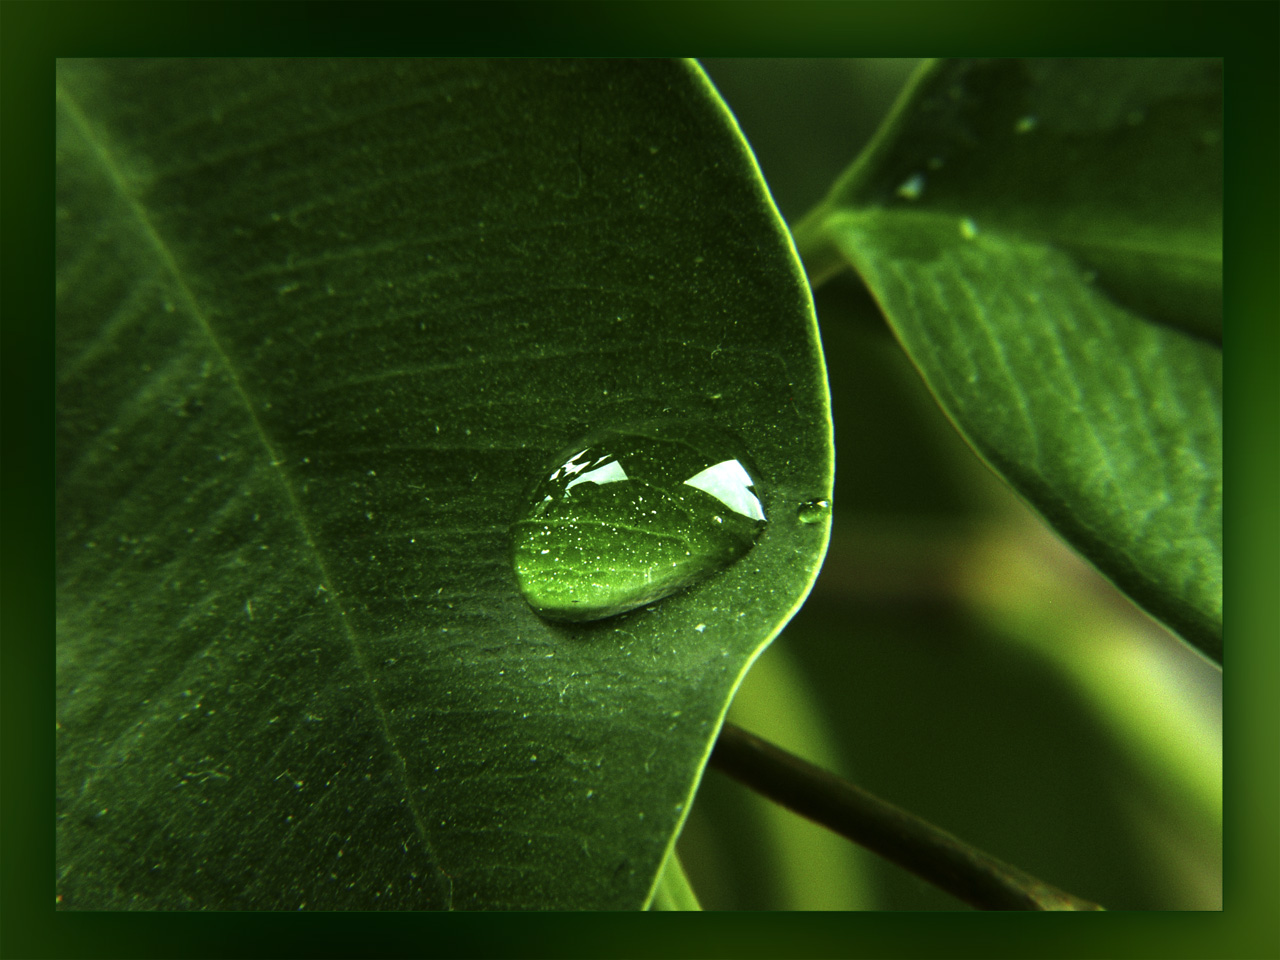
\includegraphics[width=\textwidth, scale = 0.5]{leaf.jpg}
  \caption[shorter caption for list of figures]{longer caption to explain the figure}
\end{figure}

\indent Another one pixel performance test is a comparison of the energy differences between the front and back sides of the detector. When a gamma ray interacts with the germanium crystal, an equal number of electrons and holes are created. A perfect detector would collect the same signal on both sets of contacts. Any differences in collected signal could be due to a number of factors including different amounts of impurities in the crystal, an uneven electric field, or a misalignment of the crystal axis and faces. \cite{SG09} Plotting counts vs. energy difference ($\Delta E = $ Energy$_{front} - $ Energy$_{back}$) would show any differences in collected signal. With an ideally-preforming detector these $\Delta$E plots would feature a single, well defined peak centered at zero. A comparison of pixels across the face of the detector would highlight any position-dependent deviations from equal energy collection. Gros \textit{et al.} found the most imbalance in charge collection in pixels near the guard ring. A suggestion made for suppressing this affect was collecting a signal from the guard ring to allow for identification of events that lost charge due to the pixel's location on the edge of the crystal. \cite{SG09}

(show example from Gros paper here?)

\indent The last single pixel test in the Gros paper was a plot of energy on one side vs energy on the other side for single hit events. The main feature of such a plot is a 45$^{\circ}$ line. Events falling on this line have the same signal collected on both sides of the detector. Photopeak events appear as tall peaks on this line while the Compton continuum can be clearly seen throughout the lower part of the 45$^{\circ}$ line. Events off this line didn't have the same amount of charge collected by both sides of contacts.  One will also note the presence of horizontal and vertical lines from the photopeaks nearly parallel to the axes. These tails can be explained by incomplete charge collection by a strip near the guard ring along with nearly complete collection by another strip. \cite{SG09} A superior detector will have smaller, sharper, and more symmetric tails demonstrating improved charge collection. \cite{SG09}

(pic here?)

\subsection{Double Pixel Tests}
\indent Double hit events allow for a measurement of charge sharing and loss between strips. As Gros \textit{et al.} notes, these are the events most likely to show charge sharing and charge loss and to reveal how the strips are electrically coupled. Plotting energy vs. energy and counts vs $\Delta$E for two neighboring strips on one side and one strip on the other side should show the same features as mentioned above for single hit events. Further, comparing nearest neighbor pairs with next nearest pairs should show an inverse dependence of electronic coupling on strip proximity with strips at opposite ends of the crystal displaying nearly no coupling. 

\indent An interesting effect can be seen in the plots of counts vs $\Delta$E for two hit events. An upshift in the $\Delta$E peak position brings to light the charge loss "hidden" in one hit events by the gain matching of the strips. One of the first measurements needed when turning on a new detector is a collection of single gamma data to use in gain matching the strips. Noting the position of the photopeak in each strip allows for a calibration, usually to two points, of the energy. If some of the events were actually scatters with the scattered gamma depositing energy below the level of the discriminator, the event will have a multiplicity of one. The energy deposited in the one strip will actually be less than the total energy in the incident gamma but, due to the gain matching, will be artificially raised to the energy of the incident gamma. In that way, strips can be gain matched to show a higher energy than was actually deposited. In two strip events, the effect of this calibration can be seen in a higher energy peak when the energies of two strip events are summed. The energy "lost" to the neighboring strip is effectively added back when the two strips are summed, leading to a peak higher than the incident gamma energy. It is expected that detectors showing less charge sharing will have a $\Delta$E peak closer to zero.

\indent With events where there was one hit on one side and two on the other, a plot of the energy sum ($\sum E = Energy _{two hits one side, one hit on other side}$) vs energy difference ($\Delta E = Energy _{two hits} - Energy _{one hit}$) is useful in showing the upshift in photopeak energy. \cite{SG09}

sum vs delta plots and counts vs scattering angle

\section{Tests run}
\indent

\subsection{Single Pixel Tests}
\indent

\subsection{Double Pixel Tests}
\indent went further than the Gros paper in quantitatively showing that the boron and lithium contacts behave differently. Also confirmed the performance symmetry of the PHD's detector with amorphous Ge contacts on both sides. Not much mention of the asymmetry of the boron/lithium contacts was described int eh Gros paper. Showed a difference in front/back energy plots with illumination on both sides of the Ortec detector. same tests on the NP7 showed no appreciable difference, as expected with  the symmetry of the amorphous Ge contacts.

measure the upshift in the peak in deltaE plots as a percent of incident gamma energy to get quant measure of coupling [Gros]


% \textit{italics}
% \textbf{bold}
% _{subscript}
% ^{superscript}
% $math mode$